\uuid{eAky}
\chapitre{Fonction convexe}
\niveau{L3}
\module{Optimisation}
\sousChapitre{Multiplicateurs de Lagrange}
\titre{Optimisation sous contrainte (4)}
\theme{optimisation}
\auteur{Jean-François Culus}
\datecreate{2024-10-18}
\organisation{AMSCC}
\difficulte{}
\contenu{

\question{
En vous aidant de la méthode développée à l’exercice précédent, trouver les extremums de la fonction $f(x,y)=x^3+y^3$ sous la contrainte $x^2+y^2=4$. 
}

\reponse{Posons $g(x,y)=x^2+y^2-4$, de sorte que la contrainte soit de la forme $g(x,y)=0$. 
Posons alors le Lagrangien comme étant 
$$L(x,y,\lambda)- f(x,y)-\lambda g(x,y) = x^3+y^3-\lambda (x^2+y^2-4)$$
Déterminons les points stationnaires du Lagrangien : ils vérifient donc 
$$\frac{\partial L}{\partial x} = \frac{\partial L}{\partial y} = \frac{\partial L}{\partial \lambda}=0$$
Nous obtenons alors le système suivant:
$$ 3x^2-2\lambda x=0;~~3y^2-2\lambda y=0; ~~~x^2+y^2-4=0$$
Après résolution, nous obtenons six points stationnaires possibles:
\\ $(0;2)$ correspondant à $\lambda =3$,
\\ $(0;-2)$ correspondant à $\lambda =-3$,
\\ $(2;0)$ correspondant à $\lambda = 3$,
\\ $(-2;0)$ correspondant à $\lambda =-3$
\\ $(\sqrt{2};\sqrt{2})$ correspondant à $\lambda = 3/\sqrt{2}$ 
\\ $(-\sqrt{2};-\sqrt{2})$ correspondant à $\lambda = -3/\sqrt{2}$. 

Nous allons devoir déterminer la nature des points stationnaires précédents, en examinant le signe de la forme quadratique hessienne sur les espaces tangents $T$. 
\\ Déjà, le vecteur $(u,v)$ appartient à $T$ en un point $(x_0;y_0)$ si et seulement si il est orthogonal au gradient $\nabla g(x_0,y_0)$ de $g$ au point $(x_0,y_0)$. 
Ainsi, nous obtenons pour condition pour $(u,v)\in T$:
$$ \frac{\partial g}{\partial x}(x_0;y_0) u + \frac{\partial g}{\partial y}(x_0;y_0) v=0 
~~\Leftrightarrow ~~
2x_0u+2y_0 v=0$$
Ainsi, la condition pour que $(u,v)\in T$ au point $(x_0;y_0)$ est $x_0 u+y_0v=0$.


Etudions alors la forme quadratique hessienne au point $(x_0,y_0;\lambda_0)$:
$$Q(u,v) = \frac{1}{2} \frac{\partial^2 L}{\partial x^2}(x_0;y_0;\lambda_0) u^2 + 
\frac{\partial^2 L}{\partial x \partial y}(x_0;y_0;\lambda_0) uv + 
\frac{\partial^2 L}{\partial y^2}(x_0;y_0;\lambda_0) v^2
= (3x_0-\lambda_0)u^2+(3y_0-\lambda_0)v^2$$

$\bullet$ Pour le point $(0,2)$ correspondant à $\lambda_0=3$, nous obtenons alors 
$$ (u,v)\in T \Leftrightarrow Q(u,v)=-6u^2+6v^2$$
Comme $(u,v)\in T$, nous avons que $v=0$. Il s'ensuit donc que $Q(u,0)=-6u^2$: il s'agit d'un maximum en ce point. 


$\bullet$ Pour le point $(0;-2)$: un calcul similaire conduit à un minimum en ce point. 


$\bullet$ Pour le point $(2;0)$, correspondant à $\lambda =3$: nous obtenons que 
$Q(u,v)=Q(0,v)=-6v^2$ et donc ce point est un maximum. 


$\bullet$ Pour le point $(-2;0)$ correspondant à $\lambda =-3$, nous obtenons 
$Q(u,v)=Q(0,v)=+v^2$ donc ce point est un minimum. 


$\bullet$ Pour le point $(\sqrt{2};\sqrt{2})$ correspondant à $\lambda = 3/\sqrt{2}$, nous obtenons pour contrainte de $(u,v)\in T$ que $u+v=0$ soit $u=-v$.
Il s'ensuit alors que $Q(u,v)=Q(u,-u)=6\sqrt{2}u^2>0$ et donc ce point est un minimum.


$\bullet$ Pour le point $(-\sqrt{2};-\sqrt{2})$ correspondant à $\lambda = 3/\sqrt{2}$, nous obtenons 
$Q(u,v)=Q(u,-u)=-6\sqrt{2}u^2<0$ et donc ce point est un maximum. 

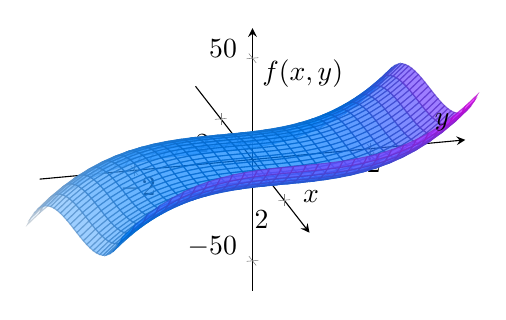
\begin{tikzpicture}
    \begin{axis}[
        xlabel={$x$},
        ylabel={$y$},
        zlabel={$f(x,y)$},
        domain=-3:3,
        y domain=-3:3,
        view={75}{30},
        samples=30,
        z buffer=sort,
        grid=both,
        axis lines=middle,
        enlargelimits,
        colormap/cool,
    ]

    % Surface of the function f(x,y) = x^3 + y^3
    \addplot3[surf, opacity=0.7] {x^3 + y^3};

    % Constraint x^2 + y^2 = 4

    \end{axis}
\end{tikzpicture}

}
}